\documentclass[a4,10pt,twoside,openright,italian,english]{book}% twoside!

\usepackage[twoside=false]{geometry}

\geometry{a4paper, margin=3cm, top=3.8cm, bindingoffset=0.4cm}

\usepackage[cam,center,a4,pdflatex,axes]{crop}
\usepackage{color,soul}
\usepackage[colorinlistoftodos]{todonotes}
\usepackage{phdthesis}
\usepackage{fancyhdr}
\usepackage{color}
\usepackage{array}
\usepackage{mdwmath}
\usepackage{mdwtab}
\usepackage{amsmath,amssymb}
\usepackage{cite}
\usepackage{graphicx}
\usepackage{listings}
\usepackage{subfig}
\usepackage{booktabs}
\usepackage{latexsym}
\usepackage{color}
\usepackage{url}
\usepackage{bnf}
\usepackage{rotating}
\usepackage{multirow}
\usepackage{phdtitle}
\usepackage{paralist}
\usepackage{bibentry}
\usepackage{xurl}
\usepackage{comment}
\usepackage[bookmarks=true,bookmarksopen=true,hidelinks]{hyperref}
\usepackage[toc,acronym]{glossaries}
\usepackage{lscape}
\usepackage{algorithmic}
\usepackage{algorithm}
\usepackage{longtable}
\usepackage[T1]{fontenc} 
\usepackage[utf8]{inputenc}
\hyphenation{}
\usepackage{mathtools}
\DeclarePairedDelimiter\ceil{\lceil}{\rceil}
\DeclarePairedDelimiter\floor{\lfloor}{\rfloor}
\usepackage{pifont}
\newcommand{\cmark}{\ding{51}}
\newcommand{\xmark}{\ding{55}}
\lstset{numbers=left, numberstyle=\tiny, stepnumber=1, numbersep=5pt}
\lstset{emph={Input,Output,if,then,else,return,end,for,begin},emphstyle={\bfseries}}


\newtheorem{Definition}{Definition}[section]

\lstset{tabsize=2,basicstyle=\footnotesize,breaklines=true}
        

\usepackage[english,italian]{babel}
\usepackage{ulem}
\normalem
\nobibliography*
\degree{Master's Degree in Cybersecurity}
\titleimage{unipi.png} %please not change

% -----------------------------------------------------------
% Please fulfil the followed fields with your data
% -----------------------------------------------------------
% -- List of author(s)
\author{Bernardini Diego, Cisternini Giovanni
% If more than one author, uncomment line(s) below (and eventtually add)
% \\Author 2
% \\Author 3
}

% -- Report Title
\title{Title}

% -- Academic year: use the format YYYY/YYYY+1
\courseyear{2024/2025}

% -----------------------------------------------------------
% Document
% -----------------------------------------------------------
% -- Main settings
\begin{document}
\selectlanguage{english}
\maketitle
\pagestyle{empty}
\cleardoublepage
\newpage
\cleardoublepage
\newpage
\pagestyle{empty}
\setcounter{page}{1}
\pagenumbering{Roman}

% -- Table of Contents (ToCs)
\tableofcontents
\cleardoublepage
\newpage
\setcounter{page}{1}
\pagenumbering{arabic}
\cleardoublepage

% -- Chapters
\chapter{Project Specifications}\label{chapter:1}
An introduction to the project, including the specifications and their analysis
\chapter{High-level Model}\label{chapter:2}
Description of the high-level model (Pyhton or C/C++ or other).
\chapter{RTL Design}\label{chapter:3}
Description of the RTL design architecture, with block diagrams, schematics (functional and/or architectural), FSM diagrams, etc ...

Figure \ref{fig:example} illustrates an example of high-level block diagram. Please, note the hierarchical organization and the usage of a blank triangle to indicate the edge-triggering logic of some blocks (i.e. blocks containing registers).

\begin{figure}[h]  % h = here, b = bottom, t = top
\centering
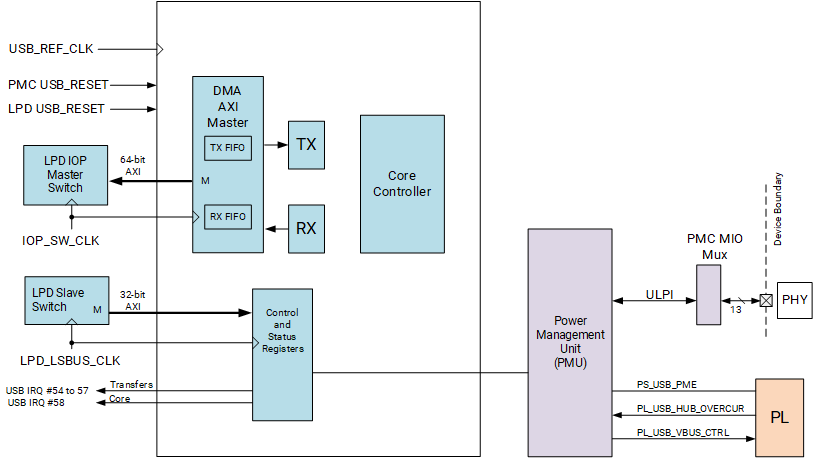
\includegraphics[width=\textwidth]{img/high_level_block_diagr.png}
\caption{Example of high-level block diagram.}\label{fig:example}
\end{figure}

In Figure \ref{fig:example}, DMA stands for Direct Access Memory, LPD indicates ... and so on. Remember to explain any symbols and/or terms and/or acronyms in figures and tables that have not been explicitly explained previously. Remember also to define each acronym before its usage!!!
\chapter{Interface Specifications and Expected Behavior}\label{chapter:4}
Describe how your module should be used in terms of how inputs should be provided (including timing) and what the corresponding output(s) would be. In practice, a kind of user manual, which may also include the waveforms at the input and/or output for several use cases (main case(s) and possible corner case(s)).
\chapter{Functional Verification}\label{chapter:5}
Describe how you tested your module, the testbench architecture, and what test(s) you performed to verify the functionality of your module according to the expected behavior described in Chapter \ref{chapter:4}
\chapter{FPGA Implementation Results}\label{chapter:6}
Describe the steps you performed on Quartus (including the FPGA device you used), the corresponding results such as resource utilization, maximum frequency, ..., and including comments on the results.

Remember that the maximum frequency is the result of the Static Timing Analysis (STA), which is optional.

Table \ref{tab:example} shows an example of table. The following link can be used to automtically generate the latex code for tables online: \url{https://www.tablesgenerator.com/}.

\begin{table}[h] % h = here, b = bottom, t = top
\centering
\caption{Example of table}\label{tab:example}
\begin{tabular}{lll}
\textbf{Heading 1} & \textbf{Heading 2} & \textbf{Heading 3} \\ \hline
Value 1.1 & Value 2.1 & Value 3.1 \\
Value 1.2 & Value 2.2 & Value 3.2
\end{tabular}
\end{table}

% -- Ending section
%\cleardoublepage
%\phantomsection
%\addcontentsline{toc}{chapter}{\bibname}
%\small

\end{document}
